\part{Data \& Methods\label{cha:data}}

%%%%%%%%%%%%%%%%%%%%%%%%%%%%%%%%%%%%%%%%%%%%%%%%%%%%%
\chapter{Data\label{cha:data}}
\section{Solar radiation measurements}
\section{Satellite data}
\section{Modelling solar radiation}
\section{photovoltaic prodution data}

%%%%%%%%%%%%%%%%%%%%%%%%%%%%%%%%%%%%%%%%%%%%%%%%%%%%%

\chapter{Methods\label{cha:methods}}

\begin{abstract}

  Para cumplir los objetivos planteados en la presente tesis es necesario el empleo de diferentes metodologías en cada uno de los capítulos de resultados, todas ellas explicadas en detalle en las correspondientes secciones. De manera general el cumplimiento de estos objetivos pasa por el análisis estadístico de las diferentes variables relacionadas con el recurso solar así como de la producción fotovoltaica, siendo esta última una estimación obtenida a partir del modelado de la misma. El análisis se realiza en escalas espacio temporales diferentes, lo que desemboca en la necesidad de utilizar adaptaciones de una misma metolodogía para cada caso.\\

  En el primer capítulo, se analizará de manera espacial la variabilidad interanual y la complementariedad del recurso solar en la Península Ibérica, para lo que se aplicarán técnicas de \textbf{clustering}. La evaluación de la productividad fotovoltaica lleva asociada la necesidad de la \textbf{modelización de un sistema fotovoltaico}.\\

  En el segundo capítulo se estudia el impacto de los aerosoles en la producitvidad fotovoltaica, esta vez en el área Euro-Mediterránea. En este caso, las \textbf{simulaciones climáticas} serán utilizadas como input del modelo fotovoltaico, creando una cadena de modelado que permita realizar un ejercicio comparativo de sensibilidad para cuantificar el papel de los aerosoles.\\
  
  Por último, se realiza el análisis del potencial fotovoltaico futuro, evaluando las tendencias y anomalías con respecto a un periodo de referencia. En este caso, se hace un \textbf{estudio multimodelo} a través de distintas simulaciones de diferentes RCMs que permita evaluar el recurso solar y se utilizan las mismas para el cálculo de la producción fotovoltaica. En este último punto vuelve a considerarse la representación del campo de AOD dentro de las simulaciones climáticas como variable determinante en las proyecciones de SSR y productividad PV.\\
  
\end{abstract} 
\section{Clustering algorithm applied to climate data}
% The culstering algorithms are design for grouping together variables and recognise patterns between them that are difficult to see at first sigth. This algorithm were first applied in ... and they have grown quickly adapting to a highly data-driven world.

% Pattern recognition: extraer objetos y agruparlos en clases. Dependiendo de las distintas disciplinas, estos objetos pueden ser muy diferentes. Se utiliza el pattern recognition en el reconocimeiento de imágenes, de palábras, ayuda en el diagnóstico, o para el análisis de bases de datos en data mining. En este último, las aplicaciones van desde la biología a las finanzas o ciencias sociales y en un data-driven world, cada vez adquiere una importancia mayor, transformando los datos en conocimiento.

% En primer lugar, se definen las características que se van a emplear como medida de similitud/similaridad utilizada para la clasificación. Una vez que estas características están definidas, los algoritmos de clustering se encargan de agrupar  estas características.

%En un mundo cada vez más movido por los datos, el reconocimiento de patrones se ha utilizado en  muchas disciplinas, desde la biología a las finanzas o las ciencias socialses, para extraer información relevante de los diferentes conjuntos de datos. Éstas técnicas, ayudan a conocer relaciones difíciles de extraer a simple vista, bien por el volumen de los datos, o por la complejidad de las mismas y la cantidad de variables involucradas. 

In a data-driven world, \textbf{pattern recognition} is being applied to many disciplines from biology to finanze through social science, in order to obtain relevant information from different datasets. These techniques help to understand relationships that are difficult to extract at a first sight, either due to the volume of the data, or the complexity of those relationships and the amount of different variables involved. Behind all the pattern recognition methods rely the simple fact of classifying objects into similar classes.\\

Depending on the a priori information about the data, it is possible to applied a \textbf{supervised} data classification/pattern recognition or \textbf{unsupervised} pattern recognition.\\

In the first stage of a supervised pattern recognition analysis there is the ability to set the measurements that will define similarity between objects, meaning the definition of the features from the dataset. The classification of different objects in the pattern recognition analysis is implemented through these features and its selection. After that, a criteria to optimally divide the features into classes is decided and applied to them. This stage is called the clasifier stage and its complexity increase with the dimensionality of the data.\\

However, if the similarity measurements can not be define first, due to unknown previous labeled data, another approach will be implemented. In that case, the task will consist in identify the similarities afterwards, from a dataset of features, applying clustering algorithms for that purpose.

\subsection{Clustering algorithms}

It is not under the scope of this work to analayse in detail all the clustering methods available, due to the vast number of them and its increasing complexity. However, it is worth it to give an overview of its classification and application in order to better understand the choice made in the study of our problem.\\

There are different types of clustering algorithms based on its application and the criteria applied to construct the clusters. The two main categories are divided in \textbf{hierarchical} and \textbf{non-hierarchical algorithms}, but there are other taxonomies based on the algorithm construction that can be used to classified different methods [ref].\\

The \textbf{hierarchical clustering algorithms} create a number of nested clusters and they can be also divided themselves in agglomerative or divisive. The first one, obtain a smaller number of cluster in each step, whereas the divisive algorithms, works on the other direction.\\

Most of these hierarchical algorithms are variants of the single-link or complete-link algorithms. They have a different way to measure similarity. In the first case, the distance between two clusters is the minimum of all the pairwise distances measured between the objects of the two clusters, in contrast, for the complete-link algorithm the distance is considered the maximum of all the pairwise distances.\\

On the orther hand, the non-hierarchical or \textbf{partitional clustering algoritm}, create a number of non-overlapping clusters. These methods could be useful when the amount of data involved is large and the construction of a dendogram, produced by the hierarchical algorithm could be computatinal expensive.\\

The partitional methods create the group of clusters using an \textbf{optimization function} which defines the similarity. The main inconvenient of these algorithms is the in advance definition of the number of clusters. Usually, the algorithm is implemented several times for a wide number of partitions and the optimum number of clusters is defined afterwards using validity indexes criteria.\\

{\color{red}{Añadir algo más sobre algoritmos partitional}}


\subsection{Clustering climate data}

As previously commented, the use of pattern recognition and in particular, the clustering analysis, has been widely used across many different disciplines. The use of these techniques to group together atmospheric variables that could help in environmental classifications is a more recent research field.[ref]\\

Historically, the climatic divisions were based mostly on the differences in vegetation types around the globe. The Koppen-Terawata classification [ref] is the most widely known climate classification and bases its divisions in obtaining the vegetation thresholds from precipitation and temperature data. Some authors had already pointed the limitations of this classification method mostly due to two aspects: the first one is that vegetation thresholds are not well defined and that could be an issue when higher spatial resoultion scales want to be defined. On the other hand, is the fact that not only precipitation and temperature are influencing the vegetation species but also other atmospheric variables like solar irradiation, as well as other environmental factors that could be related to antropoghenic emissions or waste.\\

{\color{red}{Buscar más biblio de esto}}

As these classical division are not adapted to the necessities of different fields and could be even biased, another way to geo-spatial classification is needed. In this sense it has become frequent to sucessfully use data-driven classification of different variables if it is necessary to give an spatially resolved answer. [ref]

\subsection{Applied clustering method}

In this work a clustering method is applied to classify solar irradiation due to the fact that classical climate division are only based on temperature an precipitation. The spatial pattern tha could be extract from the Koppen-Terawatta classification, can not be used for our pourpose.\\

A partitional commonly used clustering method has been selected to classify solar irradiation of the area. The \textbf{'k-means'} algorithm is easy to implement, due to the fact tha has been largely used over the literature. Moreover, the combination of a \textbf{principal component analysis} of the dataset previous to the k-means algorithm application has been proved to be an useful tool to reduce the data-dimensionality and apply the algorithm in a more efficient mamner.

\subsubsection{K-Means algorithm}

The k-means algorithm is a partitional clustering method that provide a set of partitions from the application of an optimization function, usually the euclidean distance. The algorithm initiates from a pre-defined number of clusters, 'k', and randomly selects a group of centroids equal to the number of clusters. The optimization function is applied to assign each object to one of the clusters, depending on the similarity (distance) to each of the centroids. This proccess is applied until the algorithm converges.\\

One of the limitations of these method is its dependency on the first selection of the centroids, that could lead to a local optimum instead to a global optimum. To solve these difficulty, the algorithm can be run many times to test the sensitivity of the algorithm to a different initial conditions. Another option is to use an initialization technique to select the centroids.\\

{\color{red}continuar}

\subsubsection{Principal Component Analysis}

The Principal Component Analysis, PCA [ref], consists in a decomposition of the dataset into a number of vectors whose linear combination represents the original data. The transformation of the original data into a lower dimensional space is a reduction of the dimensionality retaining the maximum of the data variance.\\

The new orthogonal system has in its first coordinate axis, the projected values of the original data that preserve most of the variance in the dataset, and it is called the principal component. The rest of principal components decrease the amount of variance explained consecutively.\\

The PCA has been applied in advance to K-means clustering algorithm among the literature [ref]. It was explained by [ref] that the reduction in dimensionality is directly linked to K-means due to the fact that the clustering membership indicators are actually the eigenvectors given by the PCA. For this reason, it has been applied before the K-means algorithm fastening the algorithm.\\

\subsubsection{Validity Index}

\subsubsection{Initialize K-Means}

\section{Regional Climate Modeling}

El sistema climático y su modelización. Modelos de circulación globales. Orígenes de los modelos de área limitada, LAM. Downscalling dinámico que pasó a ser el desarrollo de los RCM.

\section{Simulating a photovoltaic system}

In order to estimate the amount of energy produced by a photovoltaic system it is necessary first to assess the amount of energy that reach the generator surface (plane of array irradiation, $G(\alpha, \beta)$) and after this estimation, which it is not straightforward unless it is measured, the different components of the generator has to be modeled.\\

For the evaluation of the photovoltaic \textbf{energy yield}, defined as the amount of energy produced by a photovoltaic system divided by its nominal power, along this work we use the process explained below, which can be summarized in two steps:

\begin{enumerate}
\item To calculate the \textbf{effective irradiation}, $G_{eff}(\alpha, \beta)$, which is the effective irradiation after substract optical losses, due to reflection, angle of incidence ot dirtiness. The assessment of this variable has to be done from the global irradiation at the surface, $G(0)$, that can be obtain from measurements, atmospheric models or satellite datasets.
\item The second step consists in simulate the \textbf{electrical performace} of the system and estimate the power from the generator. The whole photovoltaic system includes the generator, the inverter and the transmission elements and wires.
\end{enumerate}

All the processes involved in the stage of simulating a photovoltaic system in this thesis have been made using solaR [ref], an R package that implements all the necessary functions to estimate the energy provided by the sytem.

\subsection{Global effective irradiation}

Assessing the amount of energy reaching cells of the photovoltaic generator requires to compute trackers movements, as well as the relative position between sun and panels throughout the year, a detailed description of these methods can be found in \citep{Perpinan.Marcos.ea2013}.  Once these equations are computed, the procedure is described below:

\begin{itemize}
\item First, global irradiation on the horizontal plane is decomposed in two components, \textbf{direct} and \textbf{diffuse} irradiation, Eq.\ref{GlobalIrradiation}. To estimate these quantities it is necessary to consider equations proposed by \cite{Liu1960} to characterize solar irradiation. Definition of \textit{clearness index}, Eq.\ref{K.indicedeclaridad}, is the ratio between global irradiation and extra-terrestrial irradiation at the horizontal plane. They also proposed to relate that index with the \textit{diffuse fraction}: the ratio of diffuse to global irradiation in Eq.\ref{F.diffusefraction}. This relation varies depending on the time scale. For daily values, we estimate correlation between the clearness index and the diffuse fraction using equations in \cite{Aguiar1992}. After that, the diffuse component is obtained with the definition of the \textit{diffuse fraction}, Eq.\ref{F.diffusefraction}.

\begin{equation}\label{GlobalIrradiation}
G_{d}(0) = B_{d}(0) + D_{d}(0)
\end{equation}

\nomenclature[G]{$G(0)$}{Global irradiance on the horizontal plane.}
\nomenclature[Gd]{$G_{d}(0)$}{Daily global irradiation on the horizontal plane.}
\nomenclature[D]{$D(0)$}{Diffuse irradiance on the horizontal plane.}
\nomenclature[Dd]{$D_{d}(0)$}{Daily diffuse irradiation on the horizontal plane.}
\nomenclature[B]{$B(0)$}{Direct (beam) irradiance on the horizontal plane.}
\nomenclature[Bd]{$B_{d}(0)$}{Daily direct (beam) irradiation on the horizontal plane.}


\begin{equation}\label{F.diffusefraction}
F_{D,d}=\frac{D_{d}(0)}{G_{d}(0)}
\end{equation}

\begin{equation}\label{K.indicedeclaridad}
K_{Td}=\frac{G_d(0)}{B_{0d}(0)}
\end{equation}

\item Secondly, daily irradiance has to be estimated from irradiation values. Considering low variability of solar irradiance, it is assumed that average irradiance in a short interval coincides with irradiation in that interval. Regarding equations proposed by \cite{Aguiar1992}, the ratio of the diffuse irradiance to diffuse irradiation is assumed to be equivalent to the ratio of extraterrestrial irradiance to extraterrestrial irradiation Eq.\ref{ratioB0}, and the ratio of global irradiance to daily global irradiation is followed from the same reference Eq.\ref{ratioG0}. 

\begin{equation}\label{ratioB0}
r_{D}=\frac{D(0)}{D_d(0)}=\frac{B_0(0)}{B_{0d}(0)}
\end{equation}


\begin{equation}\label{ratioG0}
r_G=\frac{G(0)}{G_d(0)}=r_D\cdot(a+b\cdot\cos(\omega))
\end{equation}

\nomenclature[Ktd]{$K_{Td}$}{Clearness index.}
\nomenclature[Fd]{$F_{D,d}$}{Diffuse fraction.}
\nomenclature[B0]{$B_0(0)$}{Direct (beam) extra-terrestrial irradiation.}
\nomenclature[B0d]{$B_{0d}(0)$}{Daily direct (beam) irradiation.}

\item The third step considers only geometrical criteria to compute the direct and diffuse irradiance components at the inclined plane.
  Diffuse irradiance is calculated with the anisotropic model proposed in \cite{hay1985estimating}. 

\item The last step estimates the effective irradiance incident on a generator subtracting dust and angle of incidence losses from the incident irradiance with the model proposed in \cite{Martin2001}.

\end{itemize}

In figure \ref{fig:algorithm_outline} the steps to assess effective irradiation at the plane-of-array is summarized.

\begin{figure}
  \centering
  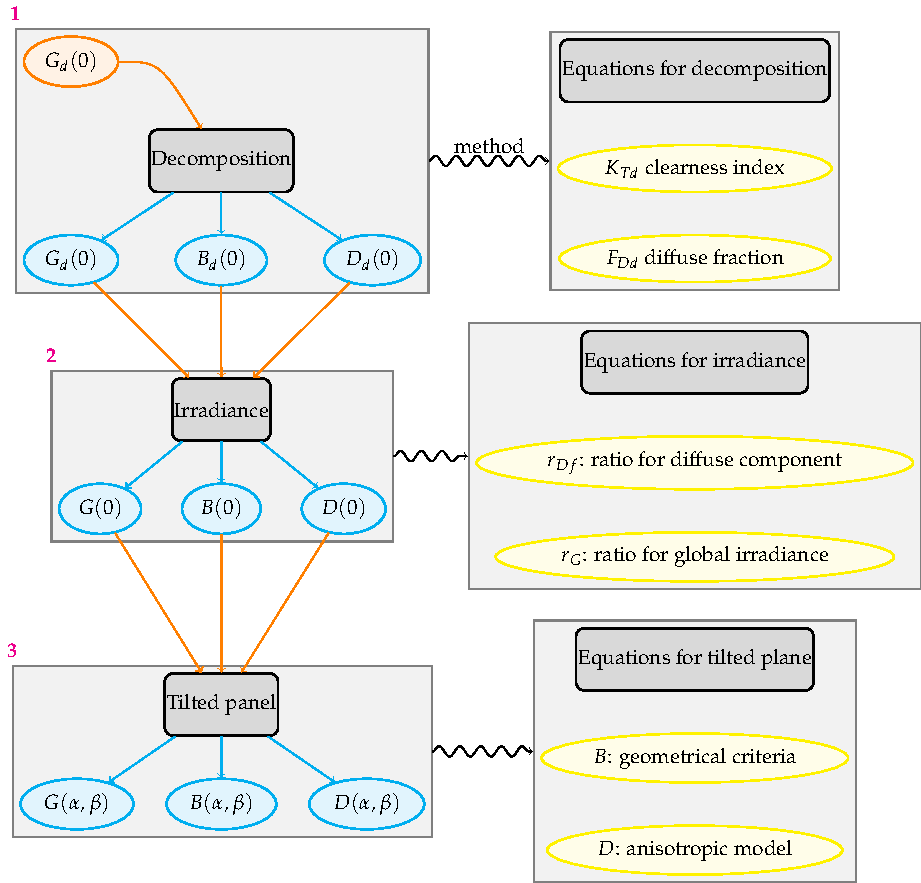
\includegraphics[width=0.6\textwidth]{figs/algorithm_outline}
  \caption{Algorithm scheme: steps on the calculation of global effective irradiation, incident irradiation at the inclined plane. Orange color means input of the calculation and blue color output or results. If a result in a previous step is used in the next one, arrows linking steps are orange. Right side of the scheme represents the method and equations needed.}
 \label{fig:algorithm_outline}
\end{figure}

\subsection{Photovoltaic energy yield}

Once the effective irradiation that reach solar cells is being assessed, the transformation into power output depends on some factors regarding the photovoltaic system. In order to estimate  potential for photovoltaic production, the term yield is defined as the energy produced by the power installed $[\si{\kilo\watthour\per\kilo\wattpeak}]$. That energy, comes from the integration in each time step of the power output of the photovoltaic system.

Considering that reach photovoltaic generator is composed of modules, the generator nominal power output is calculated by multiplying the power output of a module by the number of modules, assuming the same electric performance of all modules. 

\begin{equation}\label{Pout}
P_{out}=I_{m} \cdot V_{m}
\end{equation}

\nomenclature[P_out]{$P_{out}$}{Power output from the photovoltaic module}
\nomenclature[Im]{$I_m$}{Intensity from the photovoltaic module}
\nomenclature[Vm]{$V_m$}{Voltage of a photovoltaic module}

Ambient temperature influence cells performance. The assumption used to this assessment consider a linear relationship between cell temperature and global effective irradiation, Eq.\ref{Tcelula}. NOCT in equation \ref{Tcelula} is considered constant being the temperature of a cell when it works in determined conditions: irradiance of 800 $[\si{\watt\over\metro^2}]$ and ambient temperature of $20ºC$.

\begin{equation}\label{Tcelula}
T_c=T_a + G_{ef} \cdot \frac{NOCT-20}{800}
\end{equation}

\nomenclature[T_c]{$T_c$}{Cell temperature}
\nomenclature[T_a]{$T_a$}{Ambient temperature}
\nomenclature[G_ef]{$G_{ef}$}{Global effective irradiation}

After considering all these factors, the power output of the whole system is assessed by the consideration of a common inverter for transforming DC current into AC, also arrangement losses of the generator are included. Other systems factors that influence the performance of the photovoltaic system are shadows over the generator due to the positions of the PV modules over the land. This factor is not consider in our calculations assuming that we look for an estimation of the potential yield of an area, not the product of a real PV plant. Detailed description of the software employed to the assessment, solaR, is in \cite{Lamigueiro2012}. The process for the photovoltaic output is summarized in table \ref{tabla1} including all the steps and elements involved as explained in \cite{Perpinan2009}.

\begin{table}
  \begin{tabular}{>{\raggedright}m{6cm}>{\raggedright}m{6cm}}
    \toprule 
    Element & Method\tabularnewline
    \midrule
    PV generator & Identical modules with
    $dV_{oc}/dT_{c}=0,475\frac{\%}{\celsius}$ and $NOCT=47\celsius$. 
    The MPP point calculated as in \cite{garcia2005caracterizacion}). \tabularnewline
    \midrule
    Inverter & Efficiency equation proposed in
    \cite{jantsch1992results}:  
    \begin{equation}
      \eta_{inv}=\frac{p_{o}}{p_{o}+k_{0}^{o}+k_{1}^{o}p_{o}+k_{2}^{o}p_{o}^{2}}
    \end{equation}
    where $p_{o}=P_{ac}/P_{inv}$ is the normalized output power of the inverter. The characteristic coefficients of the
    inverters are: $k_{0}^{o}=0.01$, $k_{1}^{o}=0.025$, $k_{2}^{o}=0.05$.\tabularnewline
    \midrule
    Other losses & \begin{itemize}
    \item Average tolerance of the set of modules, $3\%$.
    \item Module parameter dispersion losses, $2\%$.
    \item Joule losses due to the wiring, $1.5\%$.
    \item Average error of the MPP algorithm of the inverter, $1\%$.
    \item Losses due to the MV transformer, $1\%$.
    \item Losses due to stops of the system, $0.5\%$.
    \end{itemize}
    \tabularnewline
    \bottomrule
  \end{tabular}
  \caption{Calculation procedure for the estimation of energy produced by a PV
    system from daily global horizontal irradiation data. Left column represents the element of the PV system and the right column the equations and methods used in each case for the efficiency of the elements.}
  \label{tabla1}
\end{table}

\nomenclature[Pinv]{$P_{inv}$}{Nominal
  power of the inverter}
\nomenclature[po]{$p_{o}$}{Normalized output power of a inverter}
\nomenclature[kinv]{$k_{i}^{o}$}{Coefficients of the
  efficiency curve of a inverter}


\section{Future projections and scenarios}

